% Rapport -- TP Techniques de compilation : du texte d'une expression régulière à l'automate
% Compiler avec pdfLaTeX (compilateur par défaut d'Overleaf).
\documentclass[12pt,a4paper]{article}

% ---------------------------------------------------------------- encodage, langue
\usepackage[utf8]{inputenc}
\usepackage[T1]{fontenc}
\IfFileExists{french.ldf}{%
  \usepackage[french]{babel}
  \frenchsetup{AutoSpacePunctuation=false, StandardItemLabels=true, StandardLists=true}
}{\usepackage[english]{babel}}

% ---------------------------------------------------------------- polices (consignes de remise)
% Texte : Times New Roman 12 ; titres : 14 ; code : Courier New 10.
% pdfLaTeX (défaut d'Overleaf) : Times et Courier (clones PostScript standard).
% XeLaTeX / LuaLaTeX : vraies polices Times New Roman / Courier New si installées.
\usepackage{iftex}
\usepackage{mathptmx}
\ifPDFTeX
  \renewcommand{\ttdefault}{pcr}
\else
  \usepackage[no-math]{fontspec}
  \IfFontExistsTF{Times New Roman}{\setmainfont{Times New Roman}}{\setmainfont{TeX Gyre Termes}}
  \IfFontExistsTF{Courier New}{\setmonofont{Courier New}}{\setmonofont{TeX Gyre Cursor}}
\fi
\linespread{1}
\usepackage{amsmath,amssymb}
\usepackage{microtype}
\usepackage[a4paper,margin=2.5cm,headheight=15pt]{geometry}
\usepackage{xcolor}
\definecolor{bleu}{HTML}{1F3B5C}
\definecolor{bleuclair}{HTML}{2E5A88}
\definecolor{fondcode}{HTML}{F4F6F9}
\definecolor{gris}{HTML}{6B7280}
\usepackage{titlesec}
\titleformat{\section}{\fontsize{14}{17}\selectfont\bfseries\color{bleu}}{\thesection.}{0.5em}{}
\titleformat{\subsection}{\fontsize{14}{17}\selectfont\bfseries\color{bleuclair}}{\thesubsection}{0.6em}{}
\titlespacing*{\section}{0pt}{1.6ex plus .5ex}{0.8ex}
\titlespacing*{\subsection}{0pt}{1.2ex plus .4ex}{0.5ex}
\usepackage{fancyhdr}
\pagestyle{fancy}
\fancyhf{}
\fancyhead[L]{\small\color{gris}TP Techniques de compilation}
\fancyhead[R]{\small\color{gris}De l'expression régulière à l'automate}
\fancyfoot[C]{\small\thepage}
\renewcommand{\headrulewidth}{0.4pt}

% ---------------------------------------------------------------- tableaux, listes, figures
\usepackage{booktabs,tabularx,array}
\usepackage{enumitem}
\setlist{itemsep=2pt,topsep=3pt}
\usepackage{graphicx}
\usepackage[font=small,labelfont={bf,color=bleu},labelsep=endash]{caption}
\usepackage{float}
\usepackage{forest}
\usepackage[most]{tcolorbox}
\usepackage[hidelinks]{hyperref}

% ---------------------------------------------------------------- code
\usepackage{listings}
\lstdefinestyle{base}{
  basicstyle=\ttfamily\fontsize{10}{12}\selectfont, columns=fixed, basewidth=0.6em, keepspaces=true,
  backgroundcolor=\color{fondcode}, frame=leftline, rulecolor=\color{bleuclair},
  framerule=1.2pt, xleftmargin=6pt, framexleftmargin=4pt, aboveskip=6pt, belowskip=6pt,
  extendedchars=false, upquote=true, breaklines=true,
  literate={′}{{$'$}}1 {ε}{{$\varepsilon$}}1 {→}{{$\rightarrow$}}1 {é}{{\'e}}1
           {è}{{\`e}}1 {à}{{\`a}}1 {…}{{\ldots}}1 {×}{{$\times$}}1
}
\lstdefinestyle{schema}{style=base}
\lstdefinestyle{py}{style=base, language=Python,
  keywordstyle=\color{bleu}\bfseries, commentstyle=\color{gris}\itshape,
  stringstyle=\color{teal!70!black}}

% ---------------------------------------------------------------- macros
\newcommand{\code}[1]{{\fontsize{10}{12}\selectfont\texttt{#1}}}
\newcommand{\eps}{\ensuremath{\varepsilon}}
\newcommand{\Prem}{\textsc{Premier}}
\newcommand{\Suiv}{\textsc{Suivant}}
\newcommand{\fr}[2]{\ensuremath{[#1\to#2]}}
\newcommand{\tok}[1]{\ensuremath{\text{\fontsize{10}{12}\selectfont\ttfamily #1}}}
\newtcolorbox{afaire}{colback=yellow!12, colframe=orange!70!black, boxrule=0pt,
  leftrule=3pt, arc=0pt, left=6pt, right=6pt, top=3pt, bottom=3pt, fontupper=\small\color{orange!40!black}}
\newcolumntype{L}{>{\raggedright\arraybackslash}X}
\newcolumntype{C}{>{\centering\arraybackslash}p}

\setlength{\emergencystretch}{4em}

\begin{document}

% ================================================================ page de garde
\begin{titlepage}
\centering
\vspace*{1.2cm}
{\fontsize{14}{17}\selectfont\color{gris} 3\textsuperscript{e} année Ingénieur Informatique --- Techniques de compilation\par}
\vspace{2.2cm}
{\color{bleu}\rule{\linewidth}{1pt}\par}
\vspace{0.5cm}
{\fontsize{24}{29}\selectfont\bfseries\color{bleu} TP Techniques de compilation\par}
\vspace{0.4cm}
{\fontsize{18}{22}\selectfont\color{bleu} Du texte d'une expression régulière à l'automate\par}
\vspace{0.3cm}
{\fontsize{12}{15}\selectfont\itshape Traduction dirigée par la syntaxe et grammaires attribuées\par}
\vspace{0.5cm}
{\color{bleu}\rule{\linewidth}{1pt}\par}
\vspace{1.2cm}
{\fontsize{14}{17}\selectfont Année universitaire 2026--2027\par}
\vspace{0.3cm}
{Rapport rendu le 25 novembre 2026 --- Langage : Python 3\par}
\vspace{1.6cm}
{\fontsize{14}{17}\selectfont\bfseries\color{bleu} Identification de l'équipe\par}
\vspace{0.4cm}
{\small
\begin{tabularx}{\linewidth}{>{\raggedright\arraybackslash}p{3.6cm} L >{\raggedright\arraybackslash}p{3.4cm}}
\toprule
Nom et prénom & Parties en charge & Parties relues \\
\midrule
ISSAOUI Edem & Étudiant 1 : analyse lexicale, partie 1 (grammaire LL(1), \Prem/\Suiv, table), partie 2 (analyseur prédictif) & Partie 4, tests, rapport \\ \addlinespace
BEN TAHER Houssem & Étudiant 2 : partie 3 (schéma de traduction, constructions de Thompson) & Parties 1 et 2 \\ \addlinespace
JAZIRI Yahia & Étudiant 3 : partie 5 (export Graphviz, simulation, interface en ligne de commande) & Partie 3 \\ \addlinespace
MTAWA Bara & Étudiant 4 : partie 4 (numérotation des états), partie 6 (jeu de tests), rapport, correction de \tok{+} et \tok{?} & Partie 5 \\
\bottomrule
\end{tabularx}\par}
\vfill
\end{titlepage}

\setcounter{page}{2}

% ================================================================ présentation et apport
\section*{Présentation et apport de l'équipe}
\addcontentsline{toc}{section}{Présentation et apport de l'équipe}

Le traducteur est écrit en Python 3 sans aucun générateur d'analyseur ni bibliothèque
d'expressions régulières. Le code (dossier \code{src/}) comporte six modules :
\code{analyseurLex.py} (jetons \code{(nature, valeur, position)}, positions comptées à partir de 0),
\code{analyseurSyntaxique.py} (une procédure par non-terminal, sans retour arrière, portant les
actions sémantiques), \code{automate.py} (les constructeurs de Thompson), \code{simulation.py}
(\eps-fermeture et reconnaissance), \code{graphviz\_export.py} (export \code{.dot}) et
\code{programme.py} (interface en ligne de commande). Un fragment d'automate est un triplet
\code{(init, fin, transitions)} ; une transition est un triplet \code{(source, étiquette, cible)},
l'étiquette \code{None} représentant \eps.

\paragraph{Notre apport.} En vérifiant les automates produits sur tous les mots courts, nous avons
découvert que la première construction de \tok{+} et \tok{?} (une simple \eps-transition ajoutée sur
les états du fragment) produisait des automates faux, par exemple \code{(ab+)?} qui acceptait
\code{b}. Nous l'avons corrigée en construisant ces deux opérateurs à partir des transitions de
l'étoile, avec deux nouveaux états, ce qui préserve l'invariant de Thompson et donne
\textbf{exactement $\boldsymbol{2n}$ états} (sections~\ref{sec:constructeurs}
et~\ref{sec:difficultes}). La numérotation des états circule comme un attribut hérité/synthétisé,
sans compteur global, et nous en donnons une preuve par récurrence (partie~4). Les messages
d'erreur indiquent la position et la liste exacte des jetons attendus. Notre jeu de tests ajoute
aux cas imposés trois expressions limites de notre invention, dix tests d'erreur, un contrôle
automatique de l'invariant de Thompson et de la borne $2n$ sur 500 expressions aléatoires et six cas
extrêmes ; nous avons vérifié qu'il détecte le défaut de la première version
(section~\ref{sec:tests}). La simulation prépare les transitions dans des dictionnaires une seule
fois par automate. Nous n'avons pas réalisé d'extension facultative : nous avons privilégié la
correction et la vérification du cœur du traducteur.

% ================================================================ PARTIE 1
\section{Partie 1 --- Grammaire LL(1)}

\subsection{\Prem{} et \Suiv{}}

$A$ n'est pas annulable, donc $\Prem(F) = \Prem(T) = \Prem(R) = \Prem(A)$. $\Suiv(R)$ contient
\tok{\$} (axiome) et \tok{)} (règle $A \to \texttt{(}\,R\,\texttt{)}$). Comme $R'$, $T'$ et $F'$
sont annulables et terminent leur règle, on obtient $\Suiv(R') = \Suiv(R)$,
$\Suiv(T) = \{\texttt{|}\} \cup \Suiv(R)$,
$\Suiv(F) = \Prem(T') \setminus \{\varepsilon\} \cup \Suiv(T)$ et
$\Suiv(A) = \{\texttt{*}, \texttt{+}, \texttt{?}\} \cup \Suiv(F)$.

\begin{table}[H]
\centering\small
\begin{tabular}{c c l l}
\toprule
Non-terminal & Annulable & \Prem & \Suiv \\
\midrule
$R$  & non & \tok{( SYMBOLE @}      & \tok{) \$} \\
$R'$ & oui & \tok{|} \eps            & \tok{) \$} \\
$T$  & non & \tok{( SYMBOLE @}      & \tok{| ) \$} \\
$T'$ & oui & \tok{( SYMBOLE @} \eps  & \tok{| ) \$} \\
$F$  & non & \tok{( SYMBOLE @}      & \tok{( SYMBOLE @ | ) \$} \\
$F'$ & oui & \tok{* + ?} \eps        & \tok{( SYMBOLE @ | ) \$} \\
$A$  & non & \tok{( SYMBOLE @}      & \tok{* + ? ( SYMBOLE @ | ) \$} \\
\bottomrule
\end{tabular}
\caption{Ensembles \Prem{} et \Suiv{} des non-terminaux.}
\end{table}

\noindent\Prem{} de chaque production (pour une production annulable, l'ensemble utilisé dans
la table est \Suiv{} de la partie gauche) :

\begin{table}[H]
\centering\small
\setlength{\tabcolsep}{4pt}
\begin{tabular}{l l @{\hspace{1.2em}} l l}
\toprule
Production & \Prem & Production & \Prem \\
\midrule
$R \to T\,R'$                       & \tok{( SYMBOLE @} & $F \to A\,F'$ & \tok{( SYMBOLE @} \\
$R' \to \texttt{|}\,T\,R'$          & \tok{|} & $F' \to \texttt{*}F' \;/\; \texttt{+}F' \;/\; \texttt{?}F'$ & \tok{*} / \tok{+} / \tok{?} \\
$R' \to \varepsilon$                & \eps{} (\Suiv : \tok{) \$}) & $F' \to \varepsilon$ & \eps{} (\Suiv : \tok{( SYMBOLE @ | ) \$}) \\
$T \to F\,T'$                       & \tok{( SYMBOLE @} & $A \to \texttt{(}\,R\,\texttt{)}$ & \tok{(} \\
$T' \to F\,T'$                      & \tok{( SYMBOLE @} & $A \to \texttt{SYMBOLE}$ & \tok{SYMBOLE} \\
$T' \to \varepsilon$                & \eps{} (\Suiv : \tok{| ) \$}) & $A \to \texttt{@}$ & \tok{@} \\
\bottomrule
\end{tabular}
\caption{\Prem{} de chaque production.}
\end{table}

\subsection{Table d'analyse prédictive}

\begin{table}[H]
\centering\small
\setlength{\tabcolsep}{5pt}
\begin{tabular}{c|ccccccccc}
\toprule
 & \tok{(} & \tok{SYMBOLE} & \tok{@} & \tok{|} & \tok{*} & \tok{+} & \tok{?} & \tok{)} & \tok{\$} \\
\midrule
$R$  & $T R'$ & $T R'$ & $T R'$ & & & & & & \\
$R'$ & & & & $\texttt{|}\,T R'$ & & & & \eps & \eps \\
$T$  & $F T'$ & $F T'$ & $F T'$ & & & & & & \\
$T'$ & $F T'$ & $F T'$ & $F T'$ & \eps & & & & \eps & \eps \\
$F$  & $A F'$ & $A F'$ & $A F'$ & & & & & & \\
$F'$ & \eps & \eps & \eps & \eps & $\texttt{*}F'$ & $\texttt{+}F'$ & $\texttt{?}F'$ & \eps & \eps \\
$A$  & $\texttt{(}R\texttt{)}$ & \tok{SYMBOLE} & \tok{@} & & & & & & \\
\bottomrule
\end{tabular}
\caption{Table LL(1) : chaque case $M[X, t]$ contient la partie droite de la production choisie ; une case vide est une erreur.}
\end{table}

Aucune case ne contient deux productions : pour chaque non-terminal à plusieurs règles, les
ensembles de la section~1.1 sont deux à deux disjoints
($R'$ : $\{\texttt{|}\} \cap \{\texttt{)}, \texttt{\$}\} = \emptyset$ ;
$T'$ : $\{\texttt{(}, \texttt{SYMBOLE}, \texttt{@}\} \cap \{\texttt{|}, \texttt{)}, \texttt{\$}\} = \emptyset$ ;
$F'$ : $\{\texttt{*}\}$, $\{\texttt{+}\}$, $\{\texttt{?}\}$ et
$\{\texttt{(}, \texttt{SYMBOLE}, \texttt{@}, \texttt{|}, \texttt{)}, \texttt{\$}\}$ disjoints ;
$A$ : $\{\texttt{(}\}$, $\{\texttt{SYMBOLE}\}$, $\{\texttt{@}\}$ disjoints).
$R$, $T$ et $F$ n'ont qu'une règle. \textbf{La grammaire est donc LL(1).}

\subsection{Grammaire de départ et concaténation implicite}

La grammaire naturelle, récursive à gauche, encode directement les priorités
(\tok{|} $<$ concaténation $<$ postfixés) et l'associativité à gauche :
\[
\begin{array}{l@{\qquad\qquad}l}
R \to R \;\texttt{|}\; T \mid T & T \to T\,F \mid F\\[2pt]
F \to F\,\texttt{*} \mid F\,\texttt{+} \mid F\,\texttt{?} \mid A &
A \to \texttt{(}\,R\,\texttt{)} \mid \texttt{SYMBOLE} \mid \texttt{@}
\end{array}
\]
Une procédure récursive pour $R \to R \;\texttt{|}\; T$ s'appellerait elle-même sans consommer
de jeton. On applique la transformation classique
$X \to X\alpha \mid \beta \;\Rightarrow\; X \to \beta X',\ X' \to \alpha X' \mid \varepsilon$,
avec $\alpha = \texttt{|}\,T$, $\beta = T$ pour $R$ ; $\alpha = F$, $\beta = F$ pour $T$ ;
$\alpha \in \{\texttt{*}, \texttt{+}, \texttt{?}\}$, $\beta = A$ pour $F$. On obtient exactement
la grammaire fournie ; le langage est inchangé.

La concaténation n'a pas d'opérateur : rien dans \code{ab} n'annonce un second facteur. Pour
choisir entre $T' \to F\,T'$ et $T' \to \varepsilon$, le seul indice est le jeton courant : on
continue si et seulement s'il peut commencer un facteur, c'est-à-dire s'il appartient à
$\Prem(F) = \{\texttt{(}, \texttt{SYMBOLE}, \texttt{@}\}$. Ce test est déterministe parce que
$\Prem(F)$ est disjoint de $\Suiv(T') = \{\texttt{|}, \texttt{)}, \texttt{\$}\}$.

\subsection{Détection des erreurs}

\begin{itemize}
\item \textbf{\code{a)}} : \code{a} est reconnu ; sur \tok{)}, $F'$, $T'$ puis $R'$
  choisissent \eps{} (cases $M[F', \texttt{)}]$, $M[T', \texttt{)}]$, $M[R', \texttt{)}]$), ce
  qui est légitime puisque \tok{)} peut suivre $R$ entre parenthèses. L'erreur n'apparaît
  qu'au contrôle de fin d'entrée après $R$ (en version tabulaire : sommet de pile \tok{\$} face
  au jeton \tok{)}).
\item \textbf{\code{a||b}} : $R'$ consomme le premier \tok{|} (case $M[R', \texttt{|}]$) puis
  appelle $T$ sur le second \tok{|} : la case \textbf{$\boldsymbol{M[T, \texttt{|}]}$ est vide},
  l'erreur est détectée à la position 2.
\end{itemize}

\noindent Messages produits par l'analyseur pour les erreurs exigées (positions à partir de 0) :

\begin{table}[H]
\centering\small
\begin{tabularx}{\linewidth}{l l L}
\toprule
Entrée & Situation & Message affiché \\
\midrule
\code{(ab} & attente de \tok{)} dans $A$ & \code{Erreur à la position 3 : ')' attendu, fin de l'expression trouvé} \\
\code{ab)} & contrôle de fin après $R$ & \code{Erreur à la position 2 : fin de l'expression attendu, ')' trouvé} \\
\code{*a} & case vide $M[R, \texttt{*}]$ & \code{Erreur à la position 0 : '(' ou un symbole ou '@' attendu, '*' trouvé} \\
\code{a||b} & case vide $M[T, \texttt{|}]$ & \code{Erreur à la position 2 : '(' ou un symbole ou '@' attendu, '|' trouvé} \\
\code{()} & case vide $M[R, \texttt{)}]$ & \code{Erreur à la position 1 : '(' ou un symbole ou '@' attendu, ')' trouvé} \\
\code{|a} & case vide $M[R, \texttt{|}]$ & \code{Erreur à la position 0 : '(' ou un symbole ou '@' attendu, '|' trouvé} \\
\code{a(} & case vide $M[A, \texttt{\$}]$ & \code{Erreur à la position 2 : '(' ou un symbole ou '@' attendu, fin de l'expression trouvé} \\
\bottomrule
\end{tabularx}
\caption{Messages d'erreur produits pour les entrées exigées par l'énoncé.}
\end{table}

% ================================================================ PARTIE 3
\section{Partie 3 --- Schéma de traduction prédictif}

\subsection{Schéma de traduction complet}

$X.h$ est le fragment déjà construit à gauche (hérité) ; $X.s$ le fragment résultat
(synthétisé). L'indice 1 distingue la seconde occurrence d'un non-terminal. Chaque action est
placée à l'endroit exact de la règle où elle s'exécute dans la procédure correspondante.

\begin{lstlisting}[style=schema]
R  → T  { R′.h := T.s }  R′  { R.s := R′.s }
R′ → '|' T  { R′1.h := union(R′.h, T.s) }  R′1  { R′.s := R′1.s }
R′ → ε  { R′.s := R′.h }
T  → F  { T′.h := F.s }  T′  { T.s := T′.s }
T′ → F  { T′1.h := concat(T′.h, F.s) }  T′1  { T′.s := T′1.s }
T′ → ε  { T′.s := T′.h }
F  → A  { F′.h := A.s }  F′  { F.s := F′.s }
F′ → '*' { F′1.h := etoile(F′.h) } F′1 { F′.s := F′1.s }
F′ → '+' { F′1.h := plus(F′.h) }   F′1 { F′.s := F′1.s }
F′ → '?' { F′1.h := option(F′.h) } F′1 { F′.s := F′1.s }
F′ → ε  { F′.s := F′.h }
A  → '(' R ')'  { A.s := R.s }
A  → SYMBOLE    { A.s := symbole(SYMBOLE.val) }
A  → '@'        { A.s := vide() }
\end{lstlisting}

Dans le code, chaque procédure $X'$ reçoit $h$ en paramètre et renvoie $s$ ; la récursion
$R' \to \texttt{|}\,T\,R'_1$ devient un appel \code{Rp(acc)} avec le fragment accumulé.

\subsection{Constructeurs de Thompson, dont \texttt{+} et \texttt{?}}\label{sec:constructeurs}

\begin{table}[H]
\centering\small
\begin{tabularx}{\linewidth}{l c L}
\toprule
Constructeur & Nouveaux états & Transitions ajoutées (\eps{} sauf indication) \\
\midrule
\code{symbole(a)}, \code{vide()} & $i, f$ & $i \xrightarrow{a} f$ \quad (resp. $i \xrightarrow{\varepsilon} f$) \\
\code{union(r, s)}  & $i, f$ & $i \to \mathrm{init}(r)$, $i \to \mathrm{init}(s)$, $\mathrm{fin}(r) \to f$, $\mathrm{fin}(s) \to f$ \\
\code{concat(r, s)} & aucun  & $\mathrm{fin}(r) \to \mathrm{init}(s)$ ; init $= \mathrm{init}(r)$, fin $= \mathrm{fin}(s)$ \\
\code{etoile(r)}    & $i, f$ & $i \to \mathrm{init}(r)$, $\mathrm{fin}(r) \to f$, $\mathrm{fin}(r) \to \mathrm{init}(r)$, $i \to f$ \\
\code{plus(r)}      & $i, f$ & $i \to \mathrm{init}(r)$, $\mathrm{fin}(r) \to f$, $\mathrm{fin}(r) \to \mathrm{init}(r)$ \quad (= étoile sans $i \to f$) \\
\code{option(r)}    & $i, f$ & $i \to \mathrm{init}(r)$, $\mathrm{fin}(r) \to f$, $i \to f$ \quad (= étoile sans la boucle) \\
\bottomrule
\end{tabularx}
\caption{Constructeurs de Thompson utilisés par les actions sémantiques.}
\end{table}

\textbf{$\boldsymbol{r^+ = r\,r^*}$} : construire $r\,r^*$ demanderait deux exemplaires de
$N(r)$. On remarque que, dans $N(r^*)$, les chemins qui passent au moins une fois par $N(r)$ sont
exactement ceux de $r^+$, et que le seul chemin qui l'évite est l'arête $i \to f$. On réutilise
donc les transitions de l'étoile \textbf{sans l'arête $\boldsymbol{i \to f}$} : un seul
exemplaire de $N(r)$, la boucle $\mathrm{fin}(r) \to \mathrm{init}(r)$ fournit les répétitions.
\textbf{$\boldsymbol{r? = r \mid \varepsilon}$} : l'union avec $N(\varepsilon)$ créerait deux
états de plus pour une simple \eps-transition. On fusionne $N(\varepsilon)$ en l'arête directe
$i \to f$ : ce sont les transitions de l'union où la branche droite est réduite à $i \to f$, soit
l'étoile \textbf{sans la boucle}. Dans les deux cas, $i$ n'a aucune transition entrante et $f$
aucune transition sortante : l'invariant de Thompson est conservé, ce qui rend la composition
sûre (voir~\ref{sec:difficultes}).

Chaque symbole, \tok{@}, \tok{|}, \tok{*}, \tok{+}, \tok{?} crée exactement deux états et la
concaténation aucun : l'automate a \textbf{exactement $\boldsymbol{2n}$ états}, ce qui garantit
la borne « au plus $2n$ ».

\subsection{Graphe de dépendances de \texttt{ab|c} : L-attribué, pas S-attribué}

\begin{figure}[H]
\centering
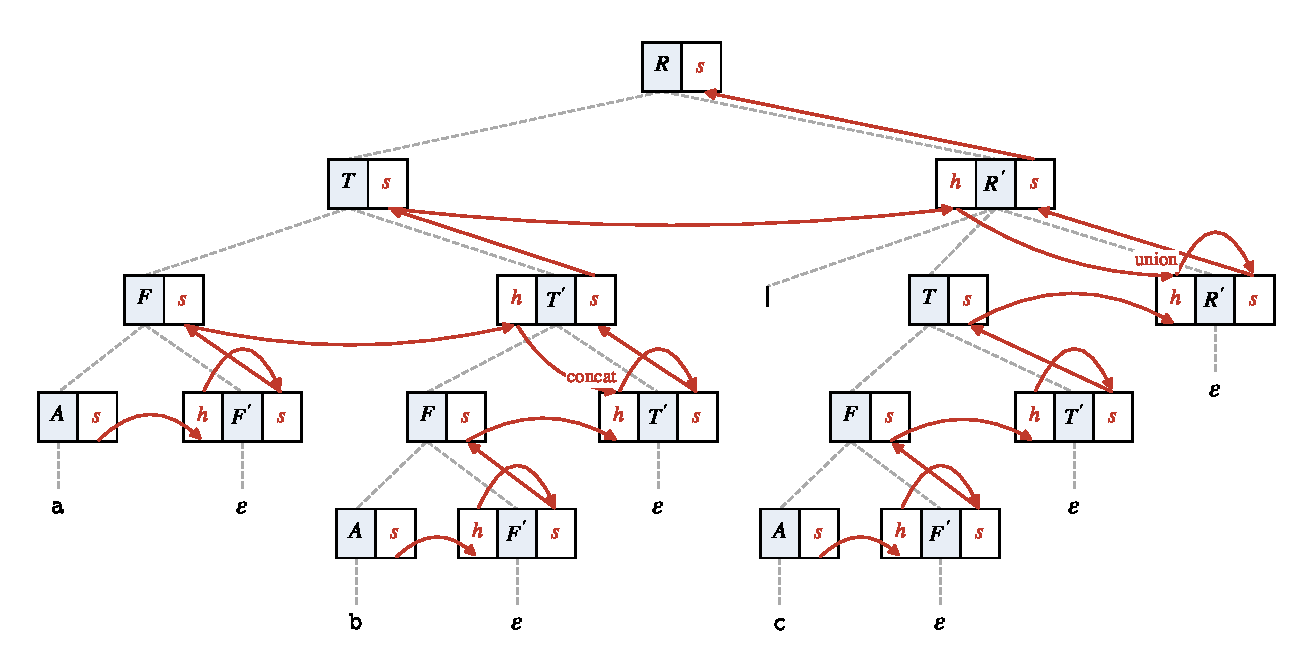
\includegraphics[width=\linewidth]{figures/dep.pdf}
\caption{Arbre de \code{ab|c} (pointillés) et dépendances entre attributs (flèches rouges).}
\label{fig:dep}
\end{figure}

Les flèches vont du fils gauche vers le frère droit ($A.s \to F'.h$, $T.s \to R'.h$), du père
vers le fils ($R'.h \to R'_1.h$) et des fils vers le père ($R'_1.s \to R'.s$). Dans chaque
règle $X \to Y_1 \dots Y_k$, un attribut hérité de $Y_i$ ne dépend que d'attributs hérités de
$X$ et d'attributs de $Y_1 \dots Y_{i-1}$ : par exemple $R'_1.h := \mathrm{union}(R'.h, T.s)$
utilise le père et le frère gauche $T$. Le schéma est donc \textbf{L-attribué} et s'évalue en
une seule passe pendant la descente récursive, de gauche à droite. Il n'est \textbf{pas
S-attribué}, car il utilise les attributs hérités $R'.h$, $T'.h$ et $F'.h$ ; ils sont
indispensables, puisque dans $R' \to \texttt{|}\,T\,R'_1$ l'opérande gauche de l'union ne se
trouve pas dans le sous-arbre de $R'$.

\subsection{Arbre annoté de \texttt{a|bc*}}

\begin{figure}[H]
\centering
\begin{forest}
  for tree={
    font=\footnotesize, align=center, inner sep=2.5pt, draw=bleuclair, rounded corners=1pt,
    fill=fondcode, l sep=9pt, s sep=6pt, edge={gris}, parent anchor=south, child anchor=north
  },
  leaf/.style={draw=none, fill=none, font=\small\ttfamily}
  [{$R$\\ $s{=}\fr{8}{9}$\\ nh=0 ns=10}
    [{$T$\\ $s{=}\fr{0}{1}$\\ nh=0 ns=2}
      [{$F$\\ $s{=}\fr{0}{1}$\\ nh=0 ns=2}
        [{$A$\\ $s{=}\fr{0}{1}$\\ nh=0 ns=2} [a, leaf]]
        [{$F'$\\ $h{=}\fr{0}{1}$\\ $s{=}\fr{0}{1}$\\ nh=2 ns=2} [\eps, leaf]]]
      [{$T'$\\ $h{=}\fr{0}{1}$\\ $s{=}\fr{0}{1}$\\ nh=2 ns=2} [\eps, leaf]]]
    [{$R'$\\ $h{=}\fr{0}{1}$\\ $s{=}\fr{8}{9}$\\ nh=2 ns=10}
      [|, leaf]
      [{$T$\\ $s{=}\fr{2}{7}$\\ nh=2 ns=8}
        [{$F$\\ $s{=}\fr{2}{3}$\\ nh=2 ns=4}
          [{$A$\\ $s{=}\fr{2}{3}$\\ nh=2 ns=4} [b, leaf]]
          [{$F'$\\ $h{=}\fr{2}{3}$\\ $s{=}\fr{2}{3}$\\ nh=4 ns=4} [\eps, leaf]]]
        [{$T'$\\ $h{=}\fr{2}{3}$\\ $s{=}\fr{2}{7}$\\ nh=4 ns=8}
          [{$F$\\ $s{=}\fr{6}{7}$\\ nh=4 ns=8}
            [{$A$\\ $s{=}\fr{4}{5}$\\ nh=4 ns=6} [c, leaf]]
            [{$F'$\\ $h{=}\fr{4}{5}$\\ $s{=}\fr{6}{7}$\\ nh=6 ns=8}
              [*, leaf]
              [{$F'$\\ $h{=}\fr{6}{7}$\\ $s{=}\fr{6}{7}$\\ nh=8 ns=8} [\eps, leaf]]]]
          [{$T'$\\ $h{=}\fr{2}{7}$\\ $s{=}\fr{2}{7}$\\ nh=8 ns=8} [\eps, leaf]]]]
      [{$R'$\\ $h{=}\fr{8}{9}$\\ $s{=}\fr{8}{9}$\\ nh=10 ns=10} [\eps, leaf]]]]
\end{forest}
\caption{Arbre annoté de \code{a|bc*} ; un fragment est noté $[\mathrm{init}\to\mathrm{fin}]$. nh/ns : numérotation (partie~4).}
\label{fig:arbre}
\end{figure}

Lecture : $A$ produit \fr01 pour \code{a} ; $R'.h$ reçoit \fr01. Dans la branche droite,
\code{b} donne \fr23, \code{c} donne \fr45, puis $F'$ applique l'étoile : \fr67. $T'$ concatène
\fr23 et \fr67 en \fr27. Enfin l'union crée \fr89, qui remonte jusqu'à $R.s$.

\subsection{Associativité à gauche avec une grammaire récursive à droite}

Les règles $R' \to \texttt{|}\,T\,R'$ et $T' \to F\,T'$ sont récursives à droite et l'arbre de
\code{a|b|c} penche à droite. L'attribut hérité rétablit pourtant l'associativité à gauche, car
il transporte vers la droite ce qui a déjà été construit. Pour \code{a|b|c} : $T$ donne
$N(a) = \fr01$ et le transmet à $R'$ ; $R'$ lit \tok{|}, construit $N(b) = \fr23$ et calcule
$\mathrm{union}(N(a), N(b)) = \fr45$, qu'il passe au $R'$ suivant ; celui-ci construit
$N(c) = \fr67$ et calcule $\mathrm{union}(\fr45, N(c)) = \fr89$. Le résultat est
\code{(a|b)|c} : dans l'automate produit, l'état initial 8 mène à 4 (le sous-automate de
\code{a|b}) et à 6 (\code{c}). Avec des attributs uniquement synthétisés
($R'.s := \mathrm{union}(T.s, R'_1.s)$), on aurait obtenu \code{a|(b|c)}. Le même mécanisme
vaut pour la concaténation via $T'.h$.

\subsection{L'opérateur le plus délicat}

C'est \textbf{\texttt{+}} (et, dans une moindre mesure, \tok{?}). La définition
$r^+ = r\,r^*$ mentionne $r$ deux fois. Réutiliser le même fragment $N(r)$ aux deux endroits
placerait les mêmes états à deux positions de l'automate et créerait de faux chemins ; le
recopier imposerait une renumérotation et casserait la borne $2n$, puisque $r$ n'est compté
qu'une fois dans $n$. Le piège est réel : notre première version ajoutait l'arête de retour
directement sur les états de $N(r)$, sans nouveaux états, et produisait des automates faux
(section~\ref{sec:difficultes}). L'étoile, elle, ajoute aussi une boucle sur $N(r)$ mais
l'enferme entre deux nouveaux états ; c'est cette précaution que nous appliquons à \tok{+} et
à \tok{?}.

% ================================================================ PARTIE 4
\section{Partie 4 --- Numérotation des états sans variable globale}\label{sec:partie4}

L'énoncé interdit tout compteur global ou statique. Le prochain numéro d'état libre devient
donc un attribut du schéma de traduction, qui circule dans l'arbre comme le fragment $h$ :
\begin{itemize}
\item $X.n$ (\textbf{hérité}) : premier numéro libre au moment où l'on commence à analyser $X$ ;
\item $X.n'$ (\textbf{synthétisé}) : premier numéro libre une fois $X$ analysé, c'est-à-dire
  après tous les états créés dans le sous-arbre de $X$.
\end{itemize}
Sur l'axiome, $R.n := 0$, et le nombre total d'états est $R.n'$. Chaque constructeur reçoit le
numéro libre et le renvoie mis à jour : symbole, vide, union, étoile, plus et option numérotent
leurs deux nouveaux états $n$ et $n+1$ et renvoient $n+2$ ; la concaténation ne crée rien et
renvoie $n$ inchangé.

\subsection{Schéma de traduction complet avec numérotation}

\begin{lstlisting}[style=schema]
R  → { T.n := R.n } T
       { R′.h := T.s ; R′.n := T.n′ } R′
       { R.s := R′.s ; R.n′ := R′.n′ }
R′ → '|' { T.n := R′.n } T
       { (R′1.h, R′1.n) := union(R′.h, T.s, T.n′) } R′1
       { R′.s := R′1.s ; R′.n′ := R′1.n′ }
R′ → ε  { R′.s := R′.h ; R′.n′ := R′.n }
T  → { F.n := T.n } F
       { T′.h := F.s ; T′.n := F.n′ } T′
       { T.s := T′.s ; T.n′ := T′.n′ }
T′ → { F.n := T′.n } F
       { (T′1.h, T′1.n) := concat(T′.h, F.s, F.n′) } T′1
       { T′.s := T′1.s ; T′.n′ := T′1.n′ }
T′ → ε  { T′.s := T′.h ; T′.n′ := T′.n }
F  → { A.n := F.n } A
       { F′.h := A.s ; F′.n := A.n′ } F′
       { F.s := F′.s ; F.n′ := F′.n′ }
F′ → '*' { (F′1.h, F′1.n) := etoile(F′.h, F′.n) } F′1
       { F′.s := F′1.s ; F′.n′ := F′1.n′ }
F′ → '+' { (F′1.h, F′1.n) := plus(F′.h, F′.n) } F′1
       { F′.s := F′1.s ; F′.n′ := F′1.n′ }
F′ → '?' { (F′1.h, F′1.n) := option(F′.h, F′.n) } F′1
       { F′.s := F′1.s ; F′.n′ := F′1.n′ }
F′ → ε  { F′.s := F′.h ; F′.n′ := F′.n }
A  → '(' { R.n := A.n } R ')' { A.s := R.s ; A.n′ := R.n′ }
A  → SYMBOLE { (A.s, A.n′) := symbole(SYMBOLE.val, A.n) }
A  → '@'     { (A.s, A.n′) := vide(A.n) }
\end{lstlisting}

Le schéma reste \textbf{L-attribué} : chaque $n$ hérité vient soit du père ($T.n := R'.n$), soit
d'un frère gauche via son $n'$ ($R'.n := T.n'$). Il s'évalue donc dans la même passe que les
fragments, sans arbre explicite.

\subsection{Mise en \oe uvre}

Dans le code, $n$ est un \textbf{paramètre} de chaque procédure et $n'$ fait partie de sa
\textbf{valeur de retour}. Chaque procédure a la forme $X(n) \to (s, n')$, et chaque procédure
primée la forme $X'(h, n) \to (s, n')$. La méthode \code{parse()} appelle \code{self.R(0)}.
Exemple de la procédure de $R'$ :

\begin{lstlisting}[style=py]
def Rp(self, h, n):                   # h = R′.h, n = R′.n
    if self.test("|"):
        self.advance()
        fragment, n1 = self.T(n)      # T.n := R′.n ; n1 = T.n′
        acc, n2 = make_union(h, fragment, n1)
                                      # états n1, n1+1 ; n2 = n1+2
        return self.Rp(acc, n2)       # R′1.h := acc ; R′1.n := n2
    if self.test(")") or self.test("EOF"):
        return h, n                   # R′.s := R′.h ; R′.n′ := R′.n
    self.error()
\end{lstlisting}

Aucun module ne contient de variable globale ni de compteur partagé. Nous avons aussi évité un
attribut d'objet du type \code{self.n}, qui serait un compteur caché équivalent à une variable
globale. Le seul état mutable de l'analyseur est l'indice du jeton courant \code{self.i}, qui
relève de l'analyse syntaxique et pas de la numérotation. Avec un numéro qui circule
explicitement, chaque analyse repart de 0 sans remise à zéro : le script de tests construit plus
de 500 automates à la suite dans le même processus.

\subsection{Exemple : numérotation de \texttt{a|bc*}}

Les états sont créés dans l'ordre où les constructeurs sont appelés, c'est-à-dire en ordre
postfixe. Les valeurs nh/ns de la figure~\ref{fig:arbre} correspondent à $n$ et $n'$ :

\begin{table}[H]
\centering\small
\begin{tabular}{c l c c c}
\toprule
Ordre & Action (nœud) & $n$ reçu & États créés & $n'$ rendu \\
\midrule
1 & \code{symbole(a)} --- $A \to \texttt{a}$ & 0 & 0, 1 & 2 \\
2 & \code{symbole(b)} --- $A \to \texttt{b}$ & 2 & 2, 3 & 4 \\
3 & \code{symbole(c)} --- $A \to \texttt{c}$ & 4 & 4, 5 & 6 \\
4 & \code{etoile}(\fr45) --- $F' \to \texttt{*}\,F'$ & 6 & 6, 7 & 8 \\
5 & \code{concat}(\fr23, \fr67) --- $T' \to F\,T'$ & 8 & aucun & 8 \\
6 & \code{union}(\fr01, \fr27) --- $R' \to \texttt{|}\,T\,R'$ & 8 & 8, 9 & 10 \\
\bottomrule
\end{tabular}
\caption{Numérotation des états de \code{a|bc*}, dans l'ordre de création.}
\end{table}

On obtient $R.n' = 10 = 2 \times 5$ pour les cinq éléments comptés \code{a}, \tok{|},
\code{b}, \code{c}, \tok{*}. L'état initial est 8 et l'état d'acceptation 9 : la dernière
opération appliquée est l'union, la plus externe.

\subsection{Propriétés garanties}

\textbf{Invariant.} Si la procédure d'un non-terminal $X$ est appelée avec $n$ et rend
$(s, n')$, alors les états de $s$ sont exactement $n, n+1, \dots, n'-1$, et $n' - n = 2k$, où
$k$ est le nombre de symboles, \tok{@}, \tok{|}, \tok{*}, \tok{+}, \tok{?} lus par $X$. Preuve
par récurrence sur l'arbre :
\begin{itemize}
\item pour $A \to \texttt{SYMBOLE}$ ou $A \to \texttt{@}$, les états sont $\{n, n+1\}$,
  $n' = n+2$ et $k = 1$ ;
\item pour une union, $T$ occupe $[n, n_1)$ par hypothèse, l'union ajoute $n_1$ et $n_1+1$, et le
  fragment de gauche ($h$) occupe les numéros précédents : l'intervalle reste contigu. Le
  raisonnement est le même pour étoile, plus et option (deux états, un opérateur) ;
\item la concaténation et les parenthèses n'ajoutent ni état ni élément compté ; les règles
  \eps{} rendent $n$ inchangé.
\end{itemize}
\textbf{Conséquences.} Deux constructeurs ne reçoivent jamais le même numéro, donc aucun état
n'est réutilisé à deux endroits. L'automate final a \textbf{exactement $\boldsymbol{2n}$ états},
numérotés de 0 à $2n-1$, ce qui garantit la propriété « au plus $2n$ états ». Le jeu de tests
vérifie les deux points (section~\ref{sec:tests}).

% ================================================================ PARTIE 5
\section{Partie 5 --- Export Graphviz et simulation}\label{sec:partie5}

Les deux fonctions de cette partie reçoivent directement le fragment construit par la partie 3 :
elles ne reconstruisent pas l'automate et n'ont pas besoin de l'arbre syntaxique.

\subsection{Export Graphviz}

Le module \code{graphviz\_export.py} contient \code{vers\_dot(fragment)}, qui construit le texte du
fichier \code{.dot}, \code{ecrire\_dot(fragment, chemin)}, qui l'écrit, et
\code{rendre\_png(chemin\_dot, chemin\_png)}, qui appelle Graphviz pour produire une image. Le graphe
est orienté de gauche à droite ; l'état initial est désigné par une flèche venant d'un point
d'entrée, l'état d'acceptation est en double cercle et les \eps-transitions portent l'étiquette
\eps. Avant l'écriture, les transitions de même source et de même cible sont regroupées sur une
seule arête (\code{a} et \code{b} deviennent \code{a,b}). Seule la conversion en image nécessite
Graphviz.

\subsection{Simulation}

La classe \code{Simulateur} de \code{simulation.py} range une seule fois les transitions dans deux
dictionnaires : les \eps-transitions par état source, et les autres transitions par état source et
par caractère. La reconnaissance d'un mot $w$ suit l'énoncé :
\begin{enumerate}
\item l'ensemble courant est l'\eps-fermeture de l'état initial ;
\item pour chaque caractère $c$ de $w$, on suit les transitions étiquetées $c$ depuis les états
  courants, puis on remplace l'ensemble courant par l'\eps-fermeture des états atteints ; si
  l'ensemble devient vide, le mot est rejeté immédiatement ;
\item le mot est accepté si l'état d'acceptation appartient à l'ensemble final.
\end{enumerate}
L'\eps-fermeture est un parcours avec une pile et un ensemble des états déjà visités : chaque état
n'est empilé qu'une fois, ce qui garantit la terminaison même en présence de cycles d'\eps{}
(\code{(a*)*}). Le mot vide est traité naturellement : aucun caractère n'est lu et l'acceptation
dépend de la fermeture initiale. La préparation coûte $O(E)$ et la reconnaissance d'un mot de
longueur $m$ coûte $O(m\,(V+E))$, pour $V$ états et $E$ transitions.

\subsection{Interface en ligne de commande}

\begin{lstlisting}[style=base]
$ python3 src/programme.py "(a|b)*abb" abb aabb ab --dot automates/abb.dot
abb : OUI
aabb : OUI
ab : NON
$ python3 src/programme.py "a?b" "" b ab
"" : NON
b : OUI
ab : OUI
$ python3 src/programme.py "a||b" x ; echo $?
Erreur à la position 2 : '(' ou un symbole ou '@' attendu, '|' trouvé
1
\end{lstlisting}

Le mot vide se passe avec \code{""}. En cas d'expression invalide, le message d'erreur est écrit sur
la sortie d'erreur et le code de retour vaut 1. L'image s'obtient ensuite avec
\code{dot -Tpng automates/abb.dot -o automates/abb.png}.

\subsection{Automates générés}

Le dossier \code{automates/} contient les fichiers \code{.dot} et \code{.png} de sept expressions
(\code{(a|b)*abb}, \code{(ab)+}, \code{a?b}, \code{a|bc*}, \code{(a*)*}, \code{a(b|c)*d},
\code{(ab+)?}), produits par \code{programme.py --dot}. Trois d'entre eux sont commentés ici.
Les états sont numérotés dans l'ordre de création des fragments, c'est-à-dire en ordre
postfixe : les sous-expressions les plus internes reçoivent les plus petits numéros, et l'état
initial n'est en général pas 0. Les arêtes parallèles sont regroupées et \eps{} est affiché
explicitement.

\begin{figure}[H]
\centering
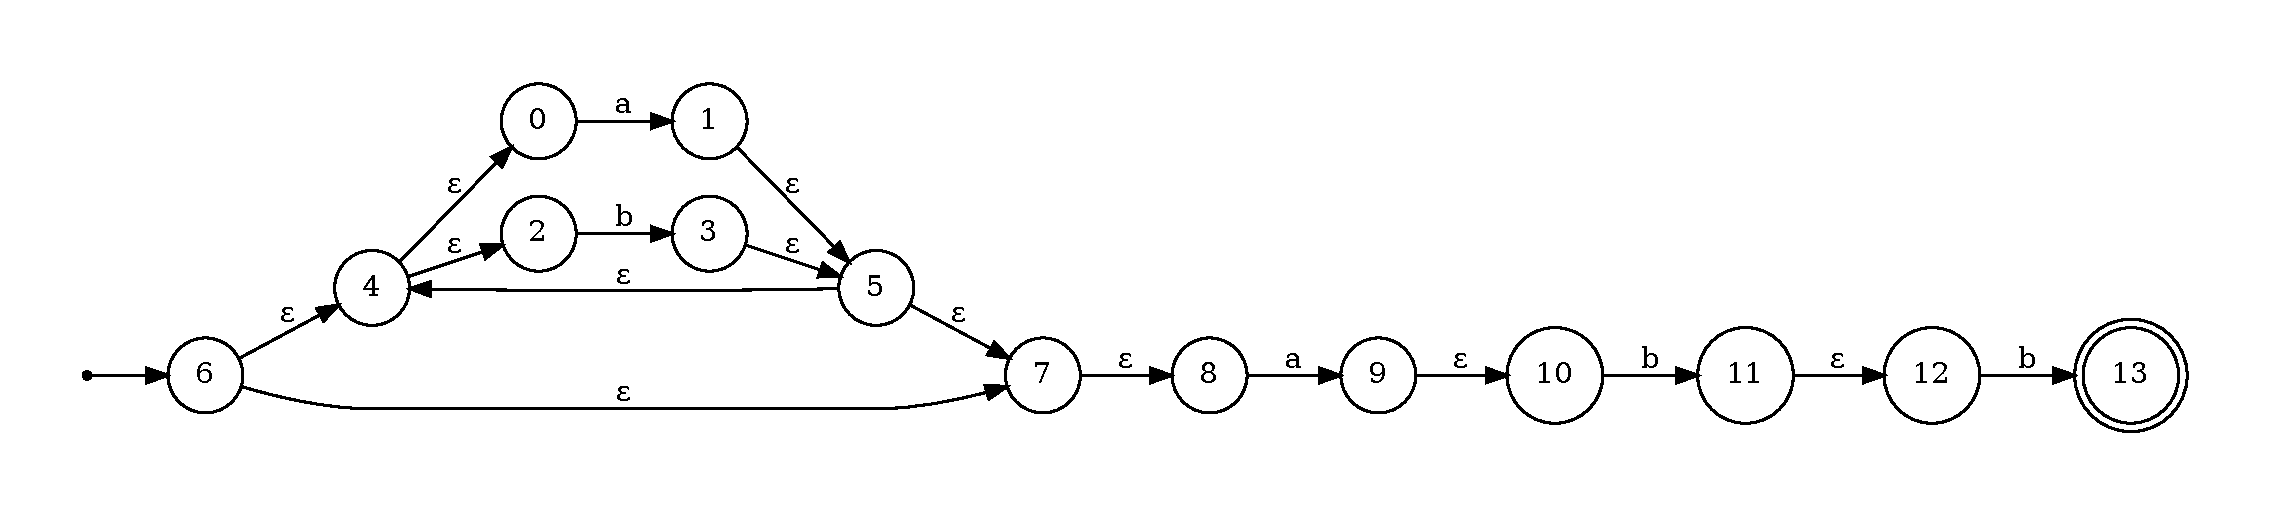
\includegraphics[width=\linewidth]{figures/abb.pdf}
\caption{\code{(a|b)*abb} : 14 états $= 2n$ avec $n = 7$ (\code{a}, \code{b}, \tok{|}, \tok{*}, \code{a}, \code{b}, \code{b}).}
\end{figure}

L'union \fr45 est construite en premier, puis enveloppée par l'étoile \fr67 : l'arête
$5 \to 4$ permet de répéter, l'arête $6 \to 7$ accepte zéro occurrence. Les trois
concaténations ne créent aucun état et ajoutent seulement $7 \to 8$, $9 \to 10$ et $11 \to 12$.
\code{abb} et \code{aabb} sont acceptés ; \code{ab} s'arrête en 11, qui n'est pas l'état
d'acceptation 13.

\begin{figure}[H]
\centering
\begin{minipage}[b]{0.48\linewidth}\centering
  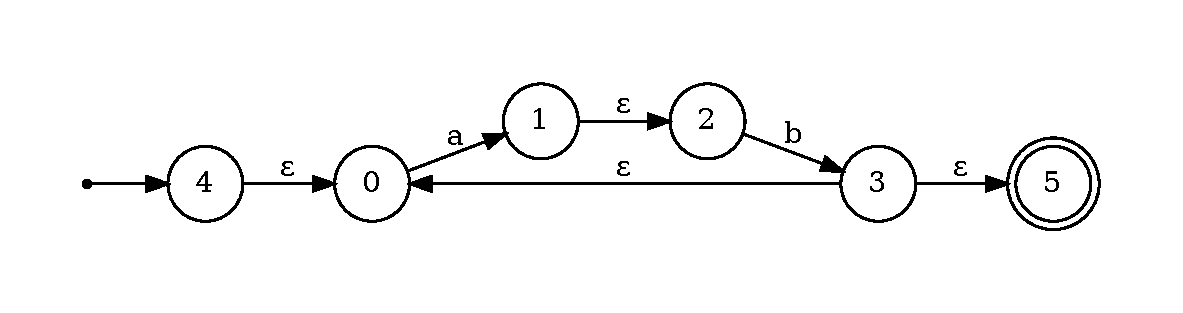
\includegraphics[width=\linewidth]{figures/ab_plus.pdf}
  \caption{\code{(ab)+} : 6 états $= 2n$ avec $n = 3$ (\code{a}, \code{b}, \tok{+}).}
\end{minipage}\hfill
\begin{minipage}[b]{0.48\linewidth}\centering
  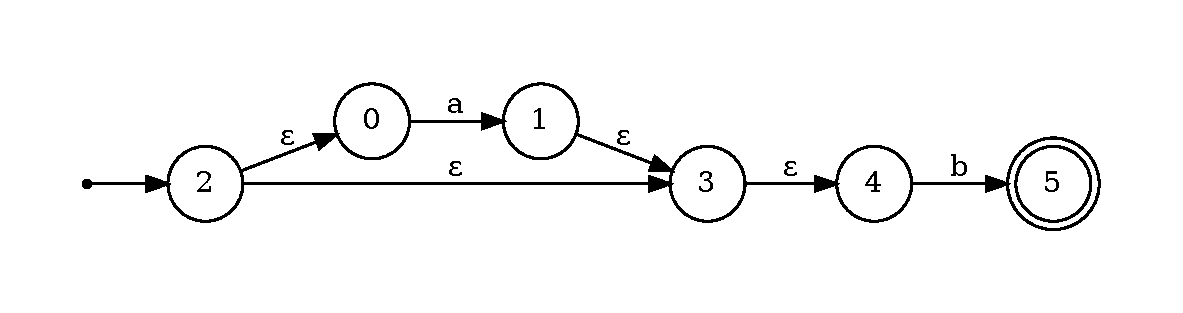
\includegraphics[width=\linewidth]{figures/a_opt_b.pdf}
  \caption{\code{a?b} : 6 états $= 2n$ avec $n = 3$ (\code{a}, \tok{?}, \code{b}).}
\end{minipage}
\end{figure}

Pour \textbf{\texttt{(ab)+}}, le fragment \code{ab} $= \fr03$ n'est pas recopié : la boucle
$3 \to 0$ permet de répéter \code{ab}, et l'absence d'arête $4 \to 5$ interdit le mot vide
(\code{ab}, \code{abab} acceptés ; \eps, \code{aba} rejetés). Pour \textbf{\texttt{a?b}},
l'arête $2 \to 3$ contourne \code{a}, et l'absence de boucle $1 \to 0$ interdit \code{aab}
(\code{b}, \code{ab} acceptés ; \code{a}, \code{aab} rejetés).

% ================================================================ TESTS
\section{Jeu de tests}\label{sec:tests}

Le jeu de tests se trouve dans \code{tests/tests.txt}. Il est exécuté par
\code{python3 tests/run\_tests.py}, depuis la racine du dépôt ; le code de retour est non nul
en cas d'échec. Chaque ligne suit le format de l'énoncé,
\code{expression ; mots acceptés ; mots rejetés}, avec \tok{@} pour le mot vide. Un test
d'erreur s'écrit \code{expression ; ERREUR ; position attendue}. Pour chaque expression
valide, le script vérifie :
\begin{itemize}
\item que chaque mot accepté est reconnu et que chaque mot rejeté est refusé ;
\item la \textbf{propriété des $\boldsymbol{2n}$ états} : le nombre d'états est au plus $2n$, et
  les états forment exactement $\{0, \dots, n'-1\}$ (partie~4) ;
\item l'\textbf{invariant de Thompson} : aucune transition n'entre dans l'état initial et aucune
  ne sort de l'état d'acceptation.
\end{itemize}
La reconnaissance utilise la fonction \code{accepte} de \code{simulation.py} (partie~5) ; si ce
module est absent, le script se rabat sur une version minimale de l'\eps-fermeture, ce qui a permis
d'écrire les tests avant la fin de la partie~5.

\subsection{Expressions valides}

\begin{table}[H]
\centering\small
\begin{tabularx}{\linewidth}{l l l L}
\toprule
Expression & Mots acceptés & Mots rejetés & Ce qui est testé \\
\midrule
\code{a}          & a                   & b, aa, @        & cas de base (imposé) \\
\code{a|b}        & a, b                & ab, @           & union (imposé) \\
\code{ab*}        & a, abbb             & b, aba, @       & priorité \tok{*} $>$ concaténation (imposé) \\
\code{(a|b)*abb}  & abb, aabb, babb     & ab, abba, @     & exemple du cours (imposé) \\
\code{(ab)+}      & ab, abab            & aba, @, b       & \tok{+} sur un groupe (imposé) \\
\code{a?b}        & b, ab               & a, aab, @       & \tok{?} (imposé) \\
\code{(a*)*}      & a, aaa, @           & b, ab           & cycle d'\eps{} (imposé) \\
\code{a(b|c)*d}   & ad, abcbd           & a, abc, @       & union sous étoile (imposé) \\
\code{@}          & @                   & a               & mot vide (imposé) \\
\midrule
\code{(ab+)?}     & @, ab, abbb         & b, bb, a, abab  & invention 1 : \tok{+} dans \tok{?} \\
\code{a*+?}       & @, a, aaaa          & b, ab           & invention 2 : postfixés enchaînés \\
\code{((a*)*)*}   & @, a, aaaa          & b, ab           & invention 3 : étoiles imbriquées \\
\midrule
\code{a|bc*}      & a, b, bc, bccc      & ac, abc, bcb, @ & priorités \tok{|} $<$ concat. $<$ \tok{*} \\
\code{(a+b)?}     & @, ab, aab          & a, aa, b, ba    & \tok{?} appliqué après un \tok{+} \\
\code{a|b|c}      & a, b, c             & ab, @, abc      & associativité de \tok{|} \\
\code{Z9|@x}      & Z9, x               & Z, 9, Zx, @     & majuscules, chiffres, \tok{@} concaténé \\
\code{(a|@)(b|@)} & @, a, b, ab         & ba, aa          & \eps{} dans deux unions \\
\code{((ab)*c)+}  & c, abc, cabc, ababcc & @, ab, abca    & étoile dans un \tok{+} \\
\bottomrule
\end{tabularx}
\caption{Expressions valides du fichier \code{tests/tests.txt} (\tok{@} : mot vide).}
\end{table}

\subsection{Justification des trois expressions de notre invention}

\begin{itemize}
\item \textbf{\texttt{(ab+)?} --- composition de \texttt{+} et \texttt{?}.} Ce cas vérifie que
  chaque opérateur respecte l'invariant de Thompson, même appliqué au résultat d'un autre
  opérateur. C'est le cas limite qui a révélé le défaut décrit en
  section~\ref{sec:difficultes} : avec des arêtes ajoutées directement sur les états de $N(r)$,
  l'arête de \tok{?} entre dans la boucle de \code{b+} et le mot \textbf{b} est accepté à tort.
\item \textbf{\texttt{a*+?} --- postfixés enchaînés.} L'énoncé précise que \code{a*+} est
  valide. Ce test vérifie la boucle
  $F' \to \texttt{*}\,F' \mid \texttt{+}\,F' \mid \texttt{?}\,F'$ de l'analyseur, et que chaque
  opérateur s'applique au fragment déjà construit (attribut hérité de $F'$). Le langage reste
  $a^*$, avec $8 = 2 \times 4$ états.
\item \textbf{\texttt{((a*)*)*} --- imbrication profonde.} Les étoiles imbriquées créent des
  cycles d'\eps{} emboîtés. Si l'\eps-fermeture ne mémorisait pas les états déjà visités, elle
  bouclerait indéfiniment. Le test vérifie aussi la numérotation avec des parenthèses
  imbriquées, un point annoncé dans le jeu de tests caché.
\end{itemize}

\subsection{Tests d'erreur}

\begin{table}[H]
\centering\small
\begin{tabularx}{\linewidth}{l c L}
\toprule
Expression & Position & Cause \\
\midrule
\code{(ab}     & 3 & parenthèse non fermée : \tok{)} attendu, fin trouvée \\
\code{ab)}     & 2 & parenthèse fermante en trop (contrôle de fin après $R$) \\
\code{*a}      & 0 & opérateur postfixé sans opérande : case vide $M[R, \texttt{*}]$ \\
\code{a||b}    & 2 & union sans opérande droit : case vide $M[T, \texttt{|}]$ \\
\code{()}      & 1 & groupe vide : case vide $M[R, \texttt{)}]$ \\
\code{|a}      & 0 & union sans opérande gauche : case vide $M[R, \texttt{|}]$ \\
\code{a(}      & 2 & groupe ouvert en fin d'entrée : case vide $M[A, \texttt{\$}]$ \\
\code{a|}      & 2 & union en fin d'entrée : case vide $M[T, \texttt{\$}]$ \\
\code{a-b}     & 1 & caractère hors alphabet \\
\code{(a|b))*} & 5 & parenthèse en trop au milieu de l'expression \\
\bottomrule
\end{tabularx}
\caption{Tests d'erreur (positions comptées à partir de 0).}
\end{table}

\subsection{Test automatique de la propriété des \texorpdfstring{$2n$}{2n} états}

En plus des 18 expressions du fichier, \code{run\_tests.py} engendre \textbf{500 expressions
aléatoires} en suivant la grammaire $R$ / $T$ / $F$ / $A$. La graine est fixée (2026), donc les
résultats sont reproductibles ; la profondeur va jusqu'à 6 niveaux de parenthèses et
l'alphabet utilisé est $\{\texttt{a}, \texttt{b}, \texttt{c}, \texttt{X}, \texttt{Y},
\texttt{0}, \texttt{9}, \texttt{@}\}$. Six cas extrêmes s'y ajoutent : 5, 20 et 40 étoiles
imbriquées \code{((\dots(a*)*\dots)*)}, une concaténation de 300 symboles, une union de 100
termes et 150 postfixés enchaînés. Pour chacun, on vérifie la borne $2n$, la numérotation
contiguë et l'invariant de Thompson.

\subsection{Résultats}

\begin{lstlisting}[style=base]
$ python3 tests/run_tests.py
...
Jeu de tests : 28/28 tests réussis
Propriété des 2n états : 506/506 expressions conformes
  (500 aléatoires, graine 2026, + 6 cas extrêmes)
\end{lstlisting}

Pour vérifier que le jeu de tests détecte bien les erreurs, nous l'avons aussi exécuté sur la
première version de \tok{+} et \tok{?} (sans nouveaux états). Résultat : \textbf{23/28} tests
du fichier et \textbf{428/506} expressions aléatoires. \code{(ab+)?} et \code{(a+b)?}
reconnaissent des mots faux. \code{(ab)+}, \code{a*+?} et \code{((ab)*c)+} violent
l'invariant de Thompson, de même que les 78 expressions aléatoires en échec, qui contiennent
toutes un \tok{+} ou un \tok{?}. Cette version respectait pourtant la borne « au plus $2n$ » ;
c'est le contrôle de l'invariant qui révèle le défaut.

% ================================================================ DIFFICULTÉS
\section{Difficultés rencontrées et choix de conception}\label{sec:difficultes}

\begin{itemize}
\item \textbf{\texttt{+} et \texttt{?} sans nouveaux états (défaut corrigé).} La première
  version de \code{make\_plus} ajoutait seulement $\mathrm{fin}(r) \to \mathrm{init}(r)$, et
  \code{make\_optional} seulement $\mathrm{init}(r) \to \mathrm{fin}(r)$, sans nouveaux états.
  Cela viole l'invariant de Thompson : après \code{b+}, l'état final de \code{b} a une
  transition sortante. Pour \code{(ab+)?}, l'arête ajoutée par \tok{?} ($0 \to 3$) entre alors
  au milieu de la boucle de \code{b+} : le chemin
  $0 \xrightarrow{\varepsilon} 3 \xrightarrow{\varepsilon} 2 \xrightarrow{b} 3$ fait accepter
  \textbf{b}, et \code{(a+b)?} acceptait \textbf{a}. La version corrigée
  (section~\ref{sec:constructeurs}) ajoute deux états par opérateur. Ce défaut a été trouvé en
  comparant les automates au langage attendu sur tous les mots de longueur $\le 4$.
\item \textbf{Messages d'erreur.} Chaque test de jeton (\code{test}) ajoute le jeton testé à
  l'ensemble \code{expected}, remis à zéro à chaque consommation. En cas d'échec, cet ensemble
  donne exactement les jetons qui auraient permis de continuer. Ils sont affichés dans un ordre
  fixe, avec une position comptée à partir de 0, comme dans l'exemple de l'énoncé.
\item \textbf{Caractères hors alphabet.} L'analyseur lexical les transmet comme jetons
  ordinaires ; l'analyseur syntaxique les rejette avec la liste des jetons attendus
  (\code{a-b} : erreur à la position 1), si bien que toutes les erreurs ont le même format.
\item \textbf{Récursivité.} \code{Rp}, \code{Tp} et \code{Fp} sont écrites en récursion directe
  pour suivre la grammaire ligne à ligne. La profondeur de la pile Python (environ 1\,000
  appels) limite donc la longueur des expressions ; une boucle \code{while} lèverait cette
  limite sans changer le schéma.
\end{itemize}

% ================================================================ RÉPARTITION
\section{Fiche de répartition}

\begin{table}[H]
\centering\small
\begin{tabularx}{\linewidth}{>{\raggedright\arraybackslash}p{3.1cm} L >{\raggedright\arraybackslash}p{3.3cm}}
\toprule
Membre & Parties écrites & Parties relues \\
\midrule
Edem Issaoui\newline{\color{gris}Étudiant 1} & \code{analyseurLex.py} ; \code{analyseurSyntaxique.py} (analyseur prédictif, messages d'erreur) ; partie 1 (\Prem/\Suiv, table LL(1), questions 1 à 4) & Partie 4, tests, rapport \\ \addlinespace
Houssem Ben Taher\newline{\color{gris}Étudiant 2} & \code{automate.py} ; actions sémantiques de \code{analyseurSyntaxique.py} ; partie 3 (schéma, graphe de dépendances, arbre annoté) & Parties 1 et 2, \code{analyseurLex.py} \\ \addlinespace
Yahia Jaziri\newline{\color{gris}Étudiant 3} & \code{graphviz\_export.py}, \code{simulation.py}, \code{programme.py} ; partie 5 (export \code{.dot}, \eps-fermeture, interface en ligne de commande) & Partie 3, \code{automate.py} \\ \addlinespace
Bara Mtawa\newline{\color{gris}Étudiant 4} & Rapport ; correction de \tok{+} et \tok{?} dans \code{automate.py} ; partie 4 ; \code{tests/tests.txt}, \code{tests/run\_tests.py} ; \code{README.txt}, \code{EQUIPE.txt} & Partie 5 \\
\bottomrule
\end{tabularx}
\end{table}

% ================================================================ RESSOURCES
\section{Ressources externes}

\begin{itemize}
\item \textbf{Support du cours} de Techniques de compilation : calcul de \Prem/\Suiv, table
  LL(1), schémas de traduction L-attribués.
\item \textbf{A. V. Aho, M. S. Lam, R. Sethi, J. D. Ullman}, \emph{Compilers: Principles,
  Techniques, and Tools}, 2\textsuperscript{e} éd., Pearson, 2006 : §3.7.4 (construction de
  Thompson), §4.4 (analyse descendante prédictive), §5.5 (définitions L-attribuées).
\item \textbf{Documentation Graphviz} (langage DOT) : attributs \code{shape}, \code{rankdir} et
  étiquettes d'arêtes.
\item \textbf{ChatGPT (OpenAI, assistant IA)}, consulté par l'Étudiant 3 (Yahia Jaziri) pour
  clarifier la méthode de simulation, proposer une organisation des fonctions de la partie 5 et
  aider à préparer des cas de test. Le code livré a ensuite été exécuté avec le jeu de tests du
  projet et les résultats ont été vérifiés.
\item \textbf{Claude (Anthropic, assistant IA)}, utilisé par l'Étudiant 4 (Bara Mtawa) pour : rédiger ce
  rapport à partir du dépôt et des documents de l'équipe ; redessiner le graphe de dépendances
  (figure~\ref{fig:dep}) ; écrire un script de vérification jetable, non inclus dans le rendu,
  qui compare les automates produits au module \code{re} de Python (utilisé seulement comme
  oracle de test) sur tous les mots de longueur $\le 4$ de $\{a, b, c, d\}$. Cette vérification
  a révélé le défaut de \tok{+} et \tok{?}, et l'outil a proposé le correctif décrit en
  section~\ref{sec:constructeurs}. Il a également servi à rédiger les parties 4 et 5 de ce
  rapport et à écrire le jeu de tests (\code{tests/tests.txt}, \code{tests/run\_tests.py}) ;
  l'erreur qu'il a commise sur les mots attendus de \code{(a+b)?} a été repérée à la première
  exécution et corrigée. Il a enfin servi à mettre le rapport en forme en \LaTeX{} selon les
  consignes de remise et à rédiger \code{README.txt} et \code{EQUIPE.txt}.
\end{itemize}

\end{document}
